\documentclass{article}
\usepackage[fontsize=14pt]{fontsize}
\usepackage{fontsetup}
\usepackage[english, russian, ukrainian]{babel}

\usepackage[margin=1.5cm]{geometry}
\usepackage{amsmath}
\usepackage{graphicx}

\begin{document}

\section*{Конденсатор з діелектриком}

Розглянемо тепер енергетичні перетворення в конденсаторах за наявності діелектрика між обкладками, вважаючи для простоти його діелектричну проникність \(\varepsilon\) постійною. Ємність конденсатора з діелектриком у \(\varepsilon\) разів більша, ніж ємність \(C\) такого ж конденсатора без діелектрика. Конденсатор із зарядом \(q\), від'єднаний від джерела живлення, має енергію \(W = q^2/(2C)\). При заповненні простору між обкладками діелектриком з проникністю \(\varepsilon\) енергія конденсатора зменшиться в \(\varepsilon\) разів: \(W' = W/\varepsilon\). Звідси відразу можна зробити висновок про те, що діелектрик втягується в електричне поле.

\begin{figure}[h]
    \centering
    % \includegraphics[width=0.6\textwidth]{figure52}
    \caption{Втягування пластини з діелектрика в плоский конденсатор}
    \label{fig:52}
\end{figure}

Втягувальна сила при незмінному заряді конденсатора зменшується в міру заповнення діелектриком простору між обкладками. Якщо на пластинах конденсатора підтримується постійна напруга, то сила, що втягує діелектрик, не залежить від довжини втягнутої частини.

Для знаходження сили, що діє на діелектрик з боку електричного поля, розглянемо втягування твердого діелектрика в горизонтально розташований конденсатор, з'єднаний з джерелом постійної напруги \(U\) (рис.~\ref{fig:52}). Нехай під дією цікавої для нас втягувальної сили \(\mathbf{F}_{\text{ел}}\) і якоїсь зовнішньої сили \(\mathbf{F}\) шматок діелектрика знаходиться в рівновазі і довжина втягнутої частини при цьому дорівнює \(x\). Припустимо, що діелектрик вдвинувся на відстань \(\Delta x\). Зовнішня сила \(F\) при цьому виконує від'ємну роботу, рівну \(F\Delta x = -F_{\text{ел}}\Delta x\). Із закону збереження енергії випливає, що зміна енергії конденсатора \(\Delta W\) дорівнює сумі роботи джерела \(A_{\text{дж}}\) і роботи зовнішньої сили \(-F_{\text{ел}}\Delta x\):
\begin{equation}
    \Delta W = A_{\text{дж}} - F_{\text{ел}} \Delta x.
\end{equation}
Як ми знаємо, \(A_{\text{дж}} = 2\Delta W\), тому рівняння (18) можна переписати у вигляді
\begin{equation}
    \Delta W = F_{\text{ел}} \Delta x.
\end{equation}
Зміна енергії конденсатора при вдвиганні діелектрика на відстань \(\Delta x\) дорівнює
\begin{equation}
    \Delta W = \frac{1}{2} U^2 \Delta C = \frac{(\varepsilon - 1)l \Delta x}{4\pi d} \frac{U^2}{2},
\end{equation}
де \(l\) --- поперечний розмір пластини.

За допомогою формул (19) і (20) знаходимо
\[
F_{\text{ел}} = \frac{\Delta W}{\Delta x} = \frac{(\varepsilon - 1)l}{4\pi d} \frac{U^2}{2},
\]
тобто сила при вдвиганні діелектрика постійна при незмінній напрузі.

Розглянемо тепер задачу про втягування рідкого діелектрика в простір між вертикальними пластинами плоского конденсатора, з'єднаного з джерелом постійної напруги \(U\) (рис.~\ref{fig:53}). Визначимо, на якій висоті \(h\) встановиться рівень рідини між пластинами при зануренні їх кінців у рідину, що має діелектричну проникність \(\varepsilon\) і густину \(\rho\), і скільки при цьому виділиться теплоти.

\begin{figure}[h]
    \centering
     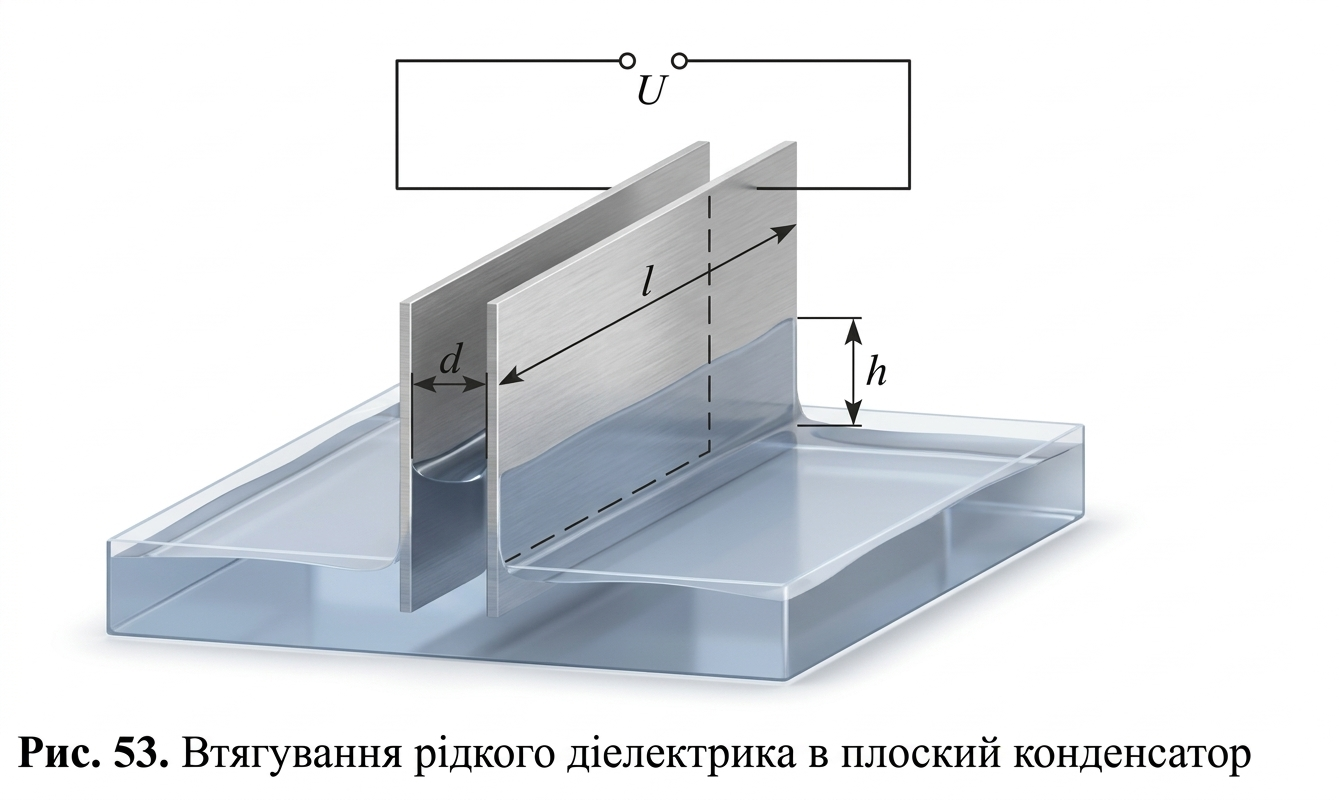
\includegraphics[width=0.75\textwidth]{figure53}
    \caption{Втягування рідкого діелектрика в плоский конденсатор}
    \label{fig:53}
\end{figure}

У стані рівноваги сила, що втягує діелектрик у простір між пластинами, врівноважується силою тяжіння \(P\), що діє на підняту рідину: \(P = \rho V g = \rho d l h g\). Для знаходження висоти підйому рідкого діелектрика прирівняємо обчислену втягувальну силу вазі рідини, що піднялася, і отримаємо
\begin{equation}
    h = \frac{(\varepsilon - 1)l U^2}{8\pi \rho g d^2}.
\end{equation}
Для знаходження теплоти, що виділилася при підйомі рідини, найпростіше виходити із закону збереження енергії. Оскільки піднятий стовп рідини перебуває у спокої, виконана джерелом робота дорівнює сумі змін енергій конденсатора і потенціальної енергії діелектрика в полі тяжіння, а також теплоти, що виділилася, \(Q\):
\[
A_{\text{дж}} = \Delta W + \frac{1}{2} m g h + Q.
\]
Враховуючи, що \(A_{\text{дж}} = 2\Delta W\), і користуючись співвідношенням (21), знаходимо
\[
Q = \frac{(\varepsilon - 1)^2 l U^4}{(4\pi)^28 \rho g d^3} = \frac{1}{2} m g h.
\]
Таким чином, робота джерела живлення розділилася навпіл: одна половина пішла на збільшення електростатичної енергії конденсатора; друга половина розділилася порівну між збільшенням потенціальної енергії діелектрика в полі тяжіння і теплотою, що виділилася. Як відбувалося виділення цієї теплоти? При зануренні пластин конденсатора в діелектрик рідина починає підніматися, набуваючи кінетичної енергії, і за інерцією проскакує положення рівноваги. Виникають коливання, які поступово затухають через в'язкість рідини, і кінетична енергія перетворюється на теплоту. Якщо в'язкість досить велика, то коливань може і не бути --- вся теплота виділяється при підйомі рідини до положення рівноваги.

\end{document}